\documentclass[crop,tikz,ifthenelse]{standalone}% 'crop' is the default for v1.0, before it was 'preview'
%\usetikzlibrary{...}% tikz package already loaded by 'tikz' option


\begin{document}
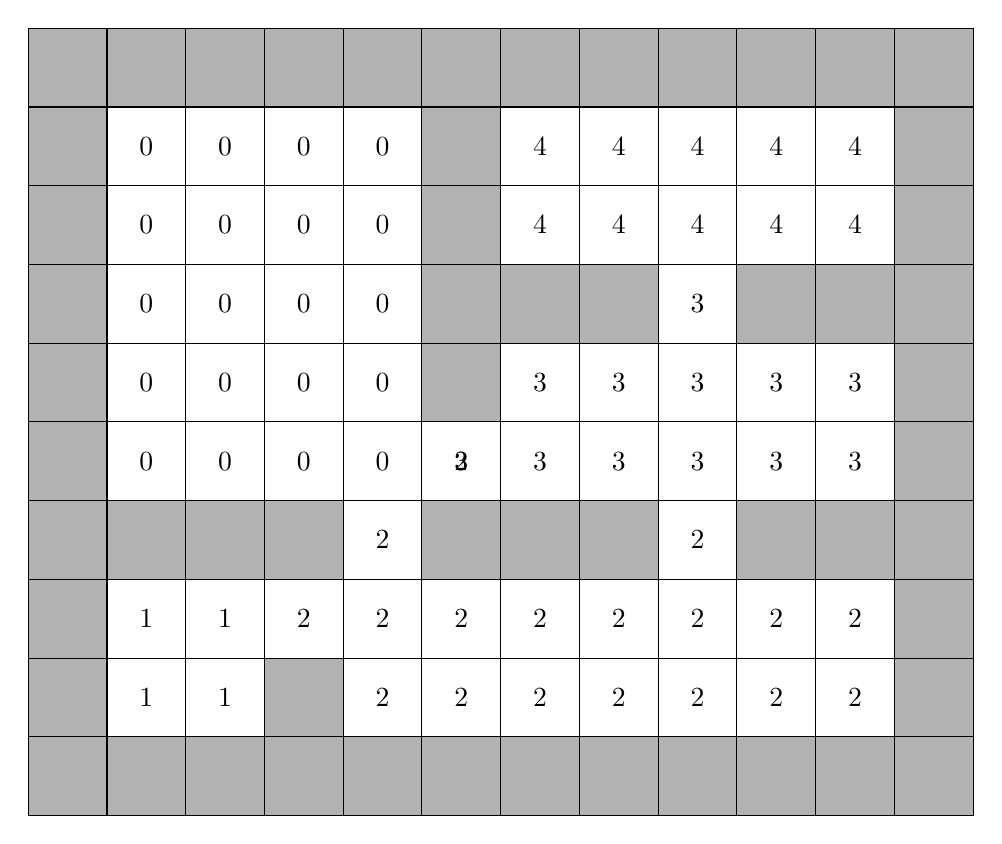
\begin{tikzpicture}[]

\newcommand{\wall}[2]{\filldraw[fill=black!30!white, draw=black] (#1,#2) rectangle (#1+1,#2+1);}
\newcommand{\area}[3]{\draw (#1,#2) rectangle (#1+1, #2+1) node[pos=.5] {#3};}

\foreach \x in {0,...,11}
  \filldraw[fill=black!30!white, draw=black] (\x,0) rectangle (\x +1, 1);

\foreach \x in {0,...,11}
  \filldraw[fill=black!30!white, draw=black] (\x,9) rectangle (\x +1, 10);

\foreach \y in {1,...,8}
  \filldraw[fill=black!30!white, draw=black] (0,\y) rectangle (1, \y+1);

\foreach \y in {1,...,8}
  \filldraw[fill=black!30!white, draw=black] (11,\y) rectangle (12, \y+1);

\foreach \x in {1,...,3}
  \filldraw[fill=black!30!white, draw=black] (\x,3) rectangle (\x+1, 4);
  
\foreach \x in {5,...,7}
  \filldraw[fill=black!30!white, draw=black] (\x,3) rectangle (\x+1, 4);

\foreach \x in {9,...,10}
  \wall{\x}{3};
  
\foreach \x in {6,...,7}
  \wall{\x}{6};

\foreach \x in {9,...,10}
  \wall{\x}{6};

\foreach \y in {5,...,8}
  \wall{5}{\y};

\wall{3}{1};


 \foreach \x in {1,...,4}
   \foreach \y in {4,...,8}
     \area{\x}{\y}{0};

\foreach \x in {1,...,2}
   \foreach \y in {1,...,2}
     \area{\x}{\y}{1};

\foreach \x in {4,...,10}
   \foreach \y in {1,...,2}
     \area{\x}{\y}{2};

\foreach \x in {6,...,10}
   \foreach \y in {4,...,5}
     \area{\x}{\y}{3};

\foreach \x in {6,...,10}
   \foreach \y in {7,...,8}
     \area{\x}{\y}{4};  

\area{5}{4}{3}; 

\area{4}{3}{2}; 
\area{3}{2}{2}; 
\area{5}{4}{2}; 
\area{8}{3}{2}; 
\area{8}{6}{3};         

% \draw (3,2) rectangle (4,3) node[pos=.5] {D};
% \draw (5,4) rectangle (6,5) node[pos=.5] {D};
% \draw (8,3) rectangle (9,4) node[pos=.5] {D};
% \draw (8,6) rectangle (9,7) node[pos=.5] {D};


\end{tikzpicture}
\end{document}
